\documentclass[border=5pt]{standalone}
\usepackage[utf8]{inputenc}
\usepackage{amsmath}
\usepackage{tikz}
\usetikzlibrary{positioning, fit, shapes}
\usetikzlibrary{chains}
\usetikzlibrary{calc}
\usetikzlibrary{decorations.pathmorphing}
\usetikzlibrary{shapes.multipart}
\usetikzlibrary{decorations,arrows}
\usetikzlibrary{decorations.pathmorphing}
\usepgflibrary{decorations.pathreplacing} 

\begin{document}

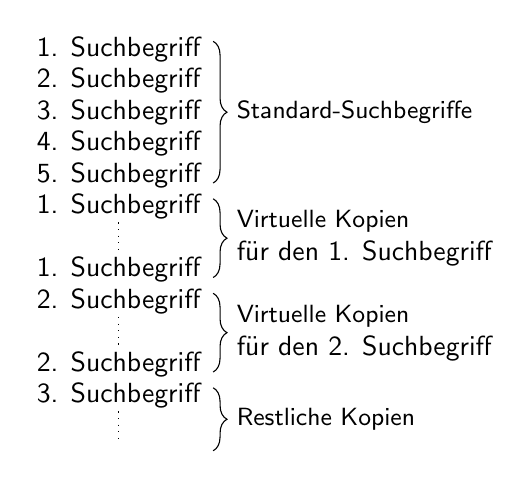
\begin{tikzpicture}[node distance=0cm, font=\sffamily]

% Manually size the picture
%\draw[opacity=0] (0, 0) -- (0, 1.7);

% Search terms
\node at (0, 5) {1. Suchbegriff};
\node at (0, 4.6) {2. Suchbegriff};
\node at (0, 4.2) {3. Suchbegriff};
\node at (0, 3.8) {4. Suchbegriff};
\node at (0, 3.4) {5. Suchbegriff};
\node at (0, 3) {1. Suchbegriff};
\draw[dotted] (0, 2.8) -- (0, 2.4);
\node at (0, 2.2) {1. Suchbegriff};
\node at (0, 1.8) {2. Suchbegriff};
\draw[dotted] (0, 1.6) -- (0, 1.2);
\node at (0, 1) {2. Suchbegriff};
\node at (0, 0.6) {3. Suchbegriff};
\draw[dotted] (0, 0.4) -- (0, 0);

% Description
\draw [decorate, decoration = {brace, amplitude=5pt}, align=left]
(1.2, 5.1) -- (1.2, 3.3) node [black, midway, right, xshift=5pt] {\small Standard-Suchbegriffe};

\draw [decorate, decoration = {brace, amplitude=5pt}, align=left]
(1.2, 3.1) -- (1.2, 2.1) node [black, midway, right, xshift=5pt] {\small Virtuelle Kopien \\ für den 1. Suchbegriff};

\draw [decorate, decoration = {brace, amplitude=5pt}, align=left]
(1.2, 1.9) -- (1.2, 0.9) node [black, midway, right, xshift=5pt] {\small Virtuelle Kopien \\ für den 2. Suchbegriff};

\draw [decorate, decoration = {brace, amplitude=5pt}, align=left]
(1.2, 0.7) -- (1.2, -0.1) node [black, midway, right, xshift=5pt] {\small Restliche Kopien};

\end{tikzpicture}

\end{document}
